\documentclass{article}

\usepackage{amsmath}
\usepackage{amssymb}
\usepackage{graphicx}
\usepackage[font=small,labelfont=bf]{caption}
\usepackage{subcaption}
\usepackage{float}
\usepackage[font={small}]{caption}
\usepackage{setspace}
\usepackage[margin=20mm]{geometry}
\usepackage{listings}
\usepackage{wrapfig}

\usepackage{fancyhdr} % Custom headers and footers
\pagestyle{fancyplain} % Makes all pages in the document conform to the custom headers and footers
\fancyhead{} % No page header - if you want one, create it in the same way as the footers below
\fancyfoot[L]{} % Empty left footer
\fancyfoot[C]{\textit{Wave Tracking Documentation}} % Empty center footer
\fancyfoot[R]{\thepage} % Page numbering for right footer
\renewcommand{\headrulewidth}{0pt} % Remove header underlines
\renewcommand{\footrulewidth}{0pt} % Remove footer underlines
\setlength{\headheight}{13.6pt} % Customize the height of the header

%\numberwithin{equation}{section} % Number equations within sections (i.e. 1.1, 1.2, 2.1, 2.2 instead of 1, 2, 3, 4)
%\numberwithin{figure}{section} % Number figures within sections (i.e. 1.1, 1.2, 2.1, 2.2 instead of 1, 2, 3, 4)
%\numberwithin{table}{section} % Number tables within sections (i.e. 1.1, 1.2, 2.1, 2.2 instead of 1, 2, 3, 4)

\newcommand{\horrule}[1]{\rule{\linewidth}{#1}} % Create horizontal rule command with 1 argument of height

\title{	
\normalfont \normalsize 
\textsc{Northumbria University: Mathematics and Information Sciences Solar group} \\ [25pt] % Your university, school and/or department name(s)
\horrule{0.5pt} \\[0.4cm] % Thin top horizontal rule
\huge Wave Tracking Code Document \\ % The assignment title
\horrule{2pt} \\[0.5cm] % Thick bottom horizontal rule
}

\author{Richard Morton*\\ Krishna Mooroogen\\ James McLaughlin} % Your name

\date{\normalsize\today} % Today's date or a custom date



\newlength\tindent
\setlength{\tindent}{\parindent}
\setlength{\parindent}{0pt}
\renewcommand{\indent}{\hspace*{\tindent}}


\begin{document}
\maketitle % Print the title

\vspace{10cm}

\begin{center}
{Version 1}\\
* Contact: richard.morton@northumbria.ac.uk 
\end{center}

\newpage
\underline{\textbf{History}}\\

Version 1 - 03/2016 - Basic operating information\\
Version 2 - 01/2019 - Updated instructions for modifications.

\vspace{2cm}

If you spot any mistakes or suggestions please email \textit{richard.morton@northumbria.ac.uk} .

\newpage
\section{Introduction}
The following describes how to run and operate software primarily developed from the measurement and analysis of kink oscillations in time-distance diagrams from solar data. However, there is scope for measurements of other features in time-distance diagrams. 

\medskip
The software was developed in part with the support of the Science and Technology Facilities Council (ST/L006243/1; ST/L006308/1).



\section{Selecting data sets}
The automated wave measurement tools are designed to analyse features in time-distance (TD) diagrams.

There are two tools available to create time-distance diagrams, \textit{diag\_slit.pro} and \textit{spline\_slit.pro}. The operation of \textit{spline\_slit.pro} is given in a separate manual.

 %#############################################################################
%#############################################################################
%\begin{figure*}[!tph]
\begin{wrapfigure}{r}{0.5\textwidth}
\centering
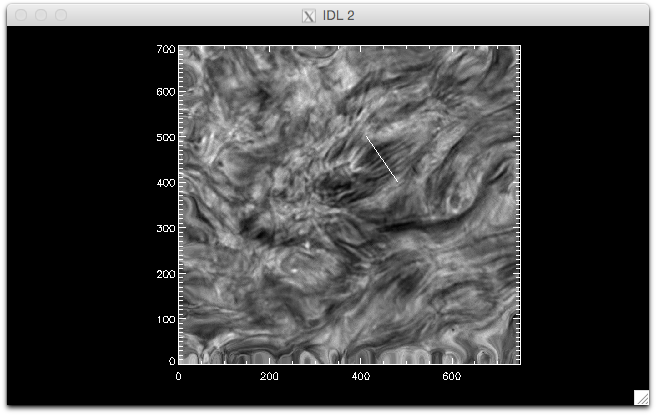
\includegraphics[scale=0.6, clip=true, viewport=4.5cm 0.cm 20.cm 14.7cm]{slit_example2.png}  
\caption{Hydrogen $\alpha$ line centre data set. The units are in pixels and the white slit shows the location of the slit from which the data for the time-distance diagram is extracted using \textit{diag\_slit}. The slit is placed across a large-scale feature composed of many fine-scale dark fibrils.
}\label{fig:slit_pick}
\vspace{-10pt}
\end{wrapfigure}
%\end{figure*}
%#############################################################################
%#############################################################################

\subsection{diag\_slit}
The \textit{diag\_slit.pro} routine is a simple point and click routine that lets you pick two data points, calculates a straight line between the
two points and extracts the intensity values along the line via cubic interpolation, doing this for all time-frames in the
data cube. \\

A typical calling procedure for \textit{diag\_slit} is:\\

\textit{IDL\textgreater diag\_slit,data\_cube,slit}\\
 
where \textit{slit} is the outputted time-distance diagram. In Figure~\ref{fig:slit_pick} a typical example of data selection is given and the output shown is shown in Figure~\ref{fig:slit_pick2}.








\section{Wave tracking}
The basic premise behind the wave tracking routine is just a simple feature finding routine. The routine identifies peaks in intensity throughout the TD diagram of interest. A peak is defined as the local maximum intensity value in a search box, whose size can be set by the user. The gradient of the slopes either side of the local maximum are used to determine whether the found local maximum is identified as a peak or not. The local maximum is required to have a positive and negative slope on the left and right hand side respectively. The user also has to select the minimum value of the gradient of the slope, i.e., a cut-off value. This value is not the same for different data sets and the user should test different values for the gradient cut-off. A gradient too large selects no points, a gradient cut-off that is too small ends up picking up the noise in the data, as well as the signal. The routine essentially scans through the TD diagram, identifying all peaks that meet the criteria. \textbf{NOTE: only positive peaks are found - so if your interested in features that have lower intensities than the background (e.g., fibrils) you will need to invert the intensities!} (we typically multiply the TD by -1 and add back the maximum image value).



 %#############################################################################
%#############################################################################
\begin{figure}[!tp]

\centering

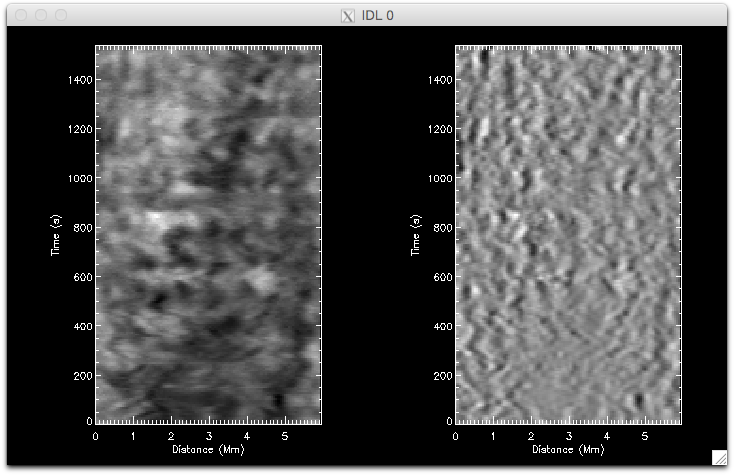
\includegraphics[scale=0.6, clip=true, viewport=0.5cm 0.cm 29.cm 16.7cm]{slit_example.png}  

\caption{Time-distance-diagrams. The left hand panel shows the intensity time-distance diagram from the slit in Figure~\ref{fig:slit_pick}. The right hand panel is an unsharp mask version of the same data, revealing more clearly the swaying of the dark fibrils.
}\label{fig:slit_pick2}

\end{figure}
%#############################################################################
%#############################################################################

\smallskip
The routine has two modes for finding the location of the peaks, one more accurate than the other. The first mode just takes the given location of maximum intensity at pixel level accuracy, and are given an error that is $\pm0.5$~pixel. This is a clearly a very coarse method.\\

 The second mode is based on the least-squares fitting of a Gaussian function to the peak in intensity, allowing for a sub-pixel estimate of the location of the intensity peak. This method inherently assumes that the intensity uncertainties are approximately Normally distributed, which is largely the case for solar data dominated by photon noise. \\

\smallskip

\subsection{{quick\_plot\_ft} }
The various wave tracking routines are made up of a number of smaller sub-routines that perform various tasks. The routine \textit{quick\_plot\_ft} is essentially a quick look routine, to test out how various input parameters influence the location and fitting of intensity peaks.\\


The basic call is: \textit{IDL\textgreater quick\_plot\_ft,td} \\

where \textit{td} is the time-distance diagram to process. This call uses the basic method for peak finding. The user will be prompted to input a gradient cut-off value. A suitable value of the gradient for different data sets will require some trial and error. In Figure~\ref{fig:slit_noth} we show the output from the routine (default plot to screen), the result is shown for the case when the cut-off is far to restrictive, and no peaks have been selected. A better selection of the gradient finds the structure, but doesn't introduce too much noise into the found peaks, an example of which is shown in Figure~\ref{fig:slit_nosm}. \\

 %#############################################################################
%#############################################################################
\begin{figure}[!tp]
\centering

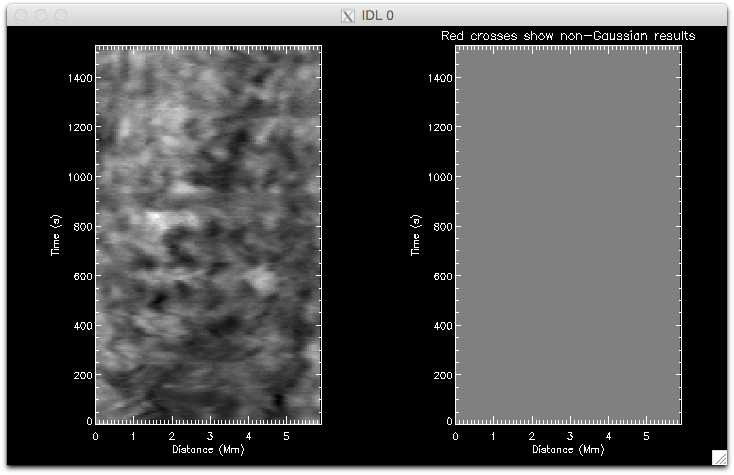
\includegraphics[scale=0.6, clip=true, viewport=0.5cm 0.cm 25.cm 16.7cm]{slit_nothing.png}  

\caption{Peak finding. The left hand panel shows the intensity time-distance diagram. The right hand panel shows the results of a harsh gradient constraint - nothing is found!
}\label{fig:slit_noth}
\end{figure}
%#############################################################################
%#############################################################################
 %#############################################################################
%#############################################################################
\begin{figure}[!tp]
\centering

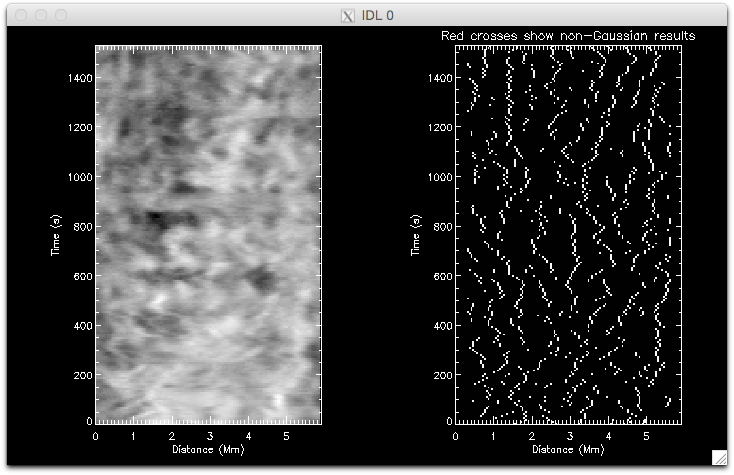
\includegraphics[scale=0.6, clip=true, viewport=0.5cm 0.cm 25.cm 16.7cm]{slit_nosmooth.png}  

\caption{Peak finding. The left hand panel shows the intensity time-distance diagram. The right hand panel shows the results of the peak location.
}\label{fig:slit_nosm}
\end{figure}
%#############################################################################
%#############################################################################

%#############################################################################
%#############################################################################
\begin{figure}[!tp]
\centering

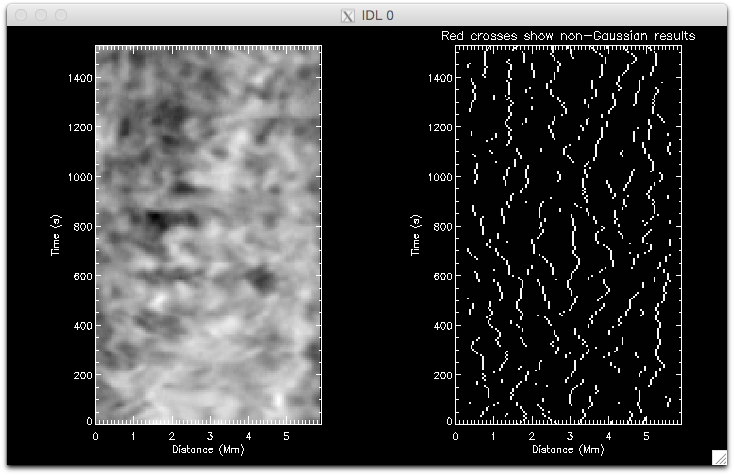
\includegraphics[scale=0.6, clip=true, viewport=0.5cm 0.cm 25.cm 16.7cm]{slit_smooth.png}  

\caption{Peak finding. The left hand panel shows the intensity time-distance diagram. The right hand panel shows the results of the peak location, with a smoothing of the TD diagram in the time-direction.
}\label{fig:slit_sm}
\end{figure}
%#############################################################################
%#############################################################################

 %#############################################################################
%#############################################################################
\begin{figure}[!tp]
\centering

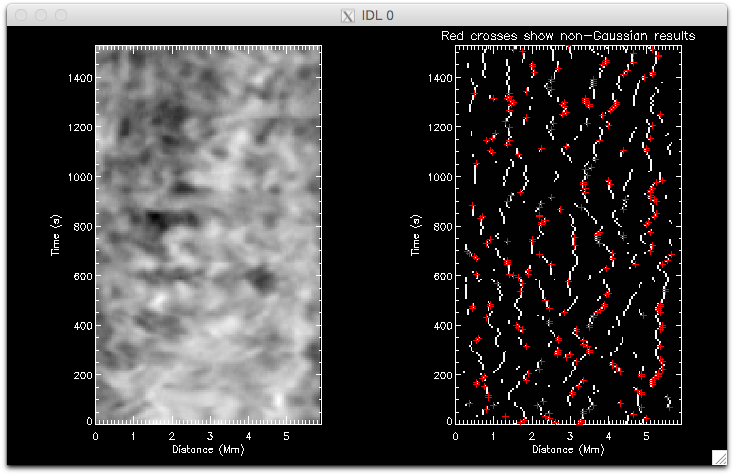
\includegraphics[scale=0.6, clip=true, viewport=0.5cm 0.cm 25.cm 16.7cm]{slit_gauss.png}  

\caption{Peak finding. The left hand panel shows the intensity time-distance diagram. The right hand panel shows the results of the peak location, using smoothed TD and the Gaussian peak location. The red crosses show where the Gaussian fit was rejected and the basic peak location is used.
}\label{fig:slit_g}
\end{figure}
%#############################################################################
%#############################################################################

In Figure~\ref{fig:slit_nosm} there is clearly the influence of noise. The influence of noise can be reduced, e.g., by averaging, smoothing, or a high-frequency noise filtering 
technique (Figure~\ref{fig:slit_sm}). \\

To test the second fitting method, the call is: \\

\textit{IDL\textgreater quick\_plot\_ft,td,/gauss,error=td\_er} \\

Here, the $td\_err$ is the uncertainties on the intensity values in the time-distance diagram. This should be calculated by 
the user using, e.g., the properties of the instrument (sensor efficiency, gain, readout noise etc.). It should be the same 
dimensions and size as $td$. The uncertainties are used 
to weight the Gaussian fit. They are required for the code to run as it makes judgements about the goodness-of-fit of the Gaussian to the peak. If the peak doesn't meet the goodness-of-fit criteria, then the location of the peak is recorded using the 
basic properties, cf the first mode.\\

 In Figure~\ref{fig:slit_g} the output window is shown for the Gaussian fitting. The red crosses show the locations where the fit of 
 the Gaussian failed to meet a list of criteria. For this example the assumed uncertainties of $0.5\%$ of the intensity value. \textbf{NOTE: careful analysis of data uncertainties is highly 
 recommended! Otherwise results will not accurately reflect the uncertainties of the peak location.} \\

There are a number of other keywords that lets you play with different parameters.

 %#############################################################################
%#############################################################################
\begin{figure}[!tp]
\centering

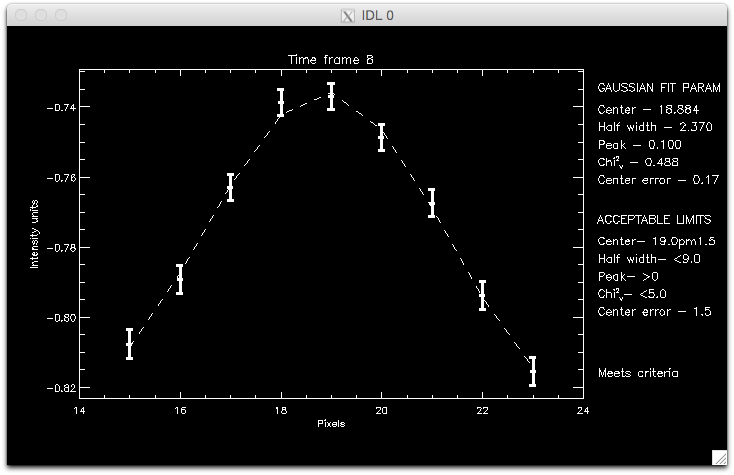
\includegraphics[scale=0.6, clip=true, viewport=0.5cm 0.cm 29.cm 16.7cm]{gauss_fit_example.png}  

\caption{Example of fitted fibril cross-section. 
}\label{fig:fit_g}
\end{figure}
%#############################################################################
%#############################################################################

 
\subsection{\textit{nuwt\_tr}}

The \textit{nuwt\_tr} routine uses the same feature finding as discussed for \textit{quick\_plot\_ft}. 
Once the peaks have been identified, an another sub-routine then `stitches' together the peaks by 
crawling through the data. The routine starts at a peak and searches forward in time for the next `local' 
peak. The search box is 5 pixels in space by 4 in time. If no pixel is found in the box, the thread is 
considered to be finished. The means small jumps in time are allowed for. \\

The basic calls for the routine are: \\

\textit{IDL\textgreater nuwt\_tr,data=td} \\

or\\

\textit{IDL\textgreater nuwt\_tr,data=td,/gauss,error=td\_er} \\

 

Here, data can be either one or many TD diagrams, in an array that is ordered as \textit{[x,t,n]}.
The user will be prompted to enter a value for the gradient cut-off and also a minimum thread length. 
The routine will then reject any thread whose length is less than that value. Further, any thread that has 
more than half of its value set to 0 will be rejected. A window will be plotted to 
screen that shows the TD and the found peaks - there is no indication at this stage of how many peak 
fittings failed for the Gaussian fit. Note, \textbf{all} peaks found are plotted - this image does not reflect 
the threads found.

\medskip
Once the fitting and stitching is complete, the user will be prompted as to whether they want to fit the 
threads. If \textit{y}, then the it takes you to an interactive fitting process, the details of which are given 
in the next sub-sub-section. Answering \textit{n} skips the fitting.

After the fitting stage, user is then asked whether they want the results to be saved. If \textit{y} is chosen 
the you will be prompted to enter a location to save the results. Once you have entered the information 
the routine will either quit (if only one TD was input) or repeat (for many TD).\\

On opening the saved file, the user will find the outputs generated by the routine are saved as structures. 
Depending on whether the threads where fitted or not, the saved outputs will either be \textit{threads} or 
\textit{threads} and \textit{threads\_fit}.

The \textit{threads} contains two extensions, \textit{threads.pos} and \textit{threads.err\_pos}, which 
give the measured location of the peaks and the uncertainty on that position. Each array has the same 
time length as the original TD. The time frames where no peak is found contain a $-1$. The remaining 
either contain the position value or a 0. The 0 corresponds to time-frames that were jumped over at the
crawling stage, i.e., no peak has been found between the time frames. \\

Note, it is up to the user to decide which found threads are worth using for further science.\\

If the user has used the internal fitting routine, then there will also be a structure called 
\textit{threads\_fit} in the idl save file. The saved data has three extensions, \textit{threads\_fit.pos}, 
\textit{threads\_fit.err\_pos}, and  \textit{threads\_fit.fit\_result}. The first two extensions contain similar 
information to \textit{threads} (although slightly modified - see wave fitting section for details). The 
extension \textit{threads\_fit.fit\_result}, predictably, contains the details related to the fitting (again, see 
fitting section for more details).


\subsection{Wave fitting}

We have updated the wave fitting part of the routine to make it more flexible. Users can now write their own function and pass this to \textit{nuwt\_tr} via the \textit{user\_func} and \textit{start} keywords. We have provided the original functions for fitting:\\
 
\begin{eqnarray}
f(t)=A_0+A_1\sin\left( \frac{2.\pi t}{A_2}-A_3\right)+tA_4,\label{eq:sinpl}\\
f(t)=A_0+A_1\sin\left( \frac{2.\pi t}{A_2}-A_3\right)\exp(-A_5t)+tA_4,\label{eq:sindp}\\
f(t)=A_0+A_1\sin\left( \frac{2.\pi t}{A_2(1+A_6t)}-A_3\right)\exp(-A_5t)+tA_4.\label{eq:sintdp}
\end{eqnarray}

The function Eq.~\ref{eq:sinpl} is the default fitting option, the others can now be selected by the above keywords. To use a non-default function you will need to provide the name of the function as a string and an array of estimates for the parameters. The array is just used for initialisation purposes and values can be altered later. The call then looks like (for model 
in Eq.~\ref{eq:sindp})

\medskip

\textit{IDL\textgreater nuwt\_tr,data=td, user\_func='damped', $start=[0.,2.,100.,0.,0.01,1.]$} \\


Note, the function chosen at the start of the routine is used for fitting all threads found! (This is obviously restrictive and we are looking to improve this aspect).\\

Once the fitting section of the routine has been entered, the routine performs a gap-filling. Any threads that have zero's in it's entries are filled. The default option for the 
filling is to give the blank entry the same value as found for the previous entry in the array and assigning it an error of $\pm1$ pixel. The large value of the error than 
essentially gives the filled location less weight in the weighted lease squares. It is these filled arrays that are then saved in \textit{threads\_fit.pos} and 
\textit{threads\_fit.err\_pos}. This fill assumes that the wave doesn't move more than 1 pixel between time-frames - how reasonable this is depends on what type of events 
you are measuring.\\

The routine will then show you which thread you are fitting, printing some text to the terminal and plotting the thread to screen. From here, there are a number of options 
for user interaction via the terminal. You will first be asked whether you would like to fit this thread. Answering \textit{n} moves on to the next thread.  Answering \textit{y},
you will then be asked if you want to change the start and end positions of the thread. This allows you focus on fitting certain portions of the thread. Answering \textit{n} moves on to the next step. Answering \textit{y} shows you the current values of time-frames it is fitting between and ask you to enter new \textit{t} and \textit{t1} values, e.g., \\

\textit{Fit this thread? - y/n y\\
Change start end of thread? - y/n y\\
Current value of t=           1 and t1=          20\\
Enter t value: 2\\
Enter t1 value: 17 }\\
 
After this, you will then be prompted about whether you want to subtract a polynomial trend line. Answering \textit{n} will skip this section. Selecting \textit{y} will then 
prompt you to enter the degree of the polynomial you wish to remove. After entering a number, a polynomial is fit to the thread and removed, with the window updated with 
the new thread. The $\chi^2$ value of the fit is printed to screen for reference.\\
 
\textit{Change polynomial degree? - y/n y\\
Fit trend - enter polynomial degree: 2\\
Chi\^{}2 of fit       10.7489\\
Is the fit good? y/n \\}

If you are happy with the subtracted polynomial then answer \textit{y}. Answering \textit{n} repeats the polynomial selection again. \textbf{Note: the removal of a polynomial 
trend before the fitting of the sinusoid will impact upon the estimated uncertainties on the fitted parameters of the sinusoid, usually underestimating the uncertainties. In 
reality, the polynomial terms should be fit with the sinusoid, rather than individually.}\\

The next section of the routine begins the fitting of the selected function (Eq.~\ref{eq:sinpl}-\ref{eq:sintdp}). The fitting is performed with a Levenberg-Marquadt algorithim 
(\textit{mpfit.pro} - cite), which requires initial guesses for the parameters to be fit. The routine has a default parameter range set, but this will likely be unsuitable for most 
cases. The user will be asked whether the initial variables should be changed, selecting \textit{n} tries the default initial values while selecting \textit{y} lets you change the start values for amplitude and period (Note, in our experience we have found that the initial values for period and amplitude have the greatest impact on the fit, hence they are the only variables allowed to change.):\\

 \textit{Initial variables: Constant=43.0000 Amplitude=1.00000 Period=20.0000 Phase=0.500000 Linear=1.00000\\
Change initial variables? y/n y\\
Enter amplitude: 2.\\
Enter period: 15.\\
\%\\
\%\\
Fitted variables      3.33458      68.1474      75.1892     -2.55123      4.85452\\
Error on fits      126.310      320.733      122.048     0.929392      17.6052\\
Chi\^{}2      75.1915\\
Repeat fitting procedure? - y/n \\
}

The fit is overplotted in the window. Should you be unhappy with the fit, selecting \textit{y} starts the process again from the selection of time-frames. This process can be 
repeated as many times as desired. Selecting \textit{n} then ends the fitting of the current thread. You are then prompted whether to save the results of the fitting. Selecting 
\textit{y} will record the fit parameters in \textit{threads\_fit.fit\_result},  selecting \textit{n} will not record the values. The routine then moves onto the next thread.\\

As mentioned, the results of the fit are stored in \textit{threads\_fit.fit\_result}. For an $n$ parameter fit, array entries correspond to:\\

\textit{fit\_result[0:n-1] - parameters\\
fit\_result[n:2n-1] - formal 1 sigma errors on parameters\\
fit\_result[2n]=chi\^{}2 for fit\\
fit\_result[2n+1]=start time from start of time-distance diagram\\
fit\_result[2n+2]=end time\\
fit\_result[2n+3]=pre-fitting used; (1)-non (2,3....)- polynomial degree\\
}


\section{To do}
The following is a list of future upgrades that may be implemented. This list is not exclusive and will be updated. If you find bugs or have suggestions, they can be added to 
the list. Further, if anybody would like to work on any of these issues please feel free!! We will be running the code through Git, so version control will be in place.\\

\begin{itemize}
\item Update $\chi^2$ cut-off for Gaussian fitting of cross-section - At present, reduced $\chi^2$ is used and set to a hard value of 5. This should be either set by a critical 
value for rejection. However, reduced $\chi^2$ is not an appropriate measure for goodness of fit for non-linear functions (cite), so implementing a Kolmogorov-Smirnov test 
may provide greater confidence.
\item Improve flexibility of fitting routine further.
\end{itemize}






\end{document}